\section{Experiments}
\label{sec:hybrid-experiments}

In this section, we conduct experiments to validate the quality of the learned hyperedges in terms of the predictive performance towards the cognition phenotype outcome. Furthermore, we conduct ablation studies to validate the key components in our model. We also analyze our results both quantitatively and qualitatively.

\subsection{Predictive Performance of Hypereges}
% \begin{algorithm}
% \begin{algorithmic}
% \STATE    $d \gets \text{an random integer between } 2 \text{ and } 30. $

% \STATE $\mathcal{H} \gets \{\}$
% \FOR{$i = 1:d$}
% \STATE $h \gets \text{randomly sample } d \text{ nodes}$
% \STATE $\mathcal{H} \gets \mathcal{H} \cup \{h\}$
% \ENDFOR

% \FORALL{$h$ in $H$}
% \FORALL{node in $h$}

% \STATE $w \gets U(0, 1)$
% \STATE $x \gets U(0, 2w)$
% \STATE $y \gets y + $

% \ENDFOR
% \ENDFOR

% \end{algorithmic}

% \caption{The procedure to construct the synthetic dataset.}
% \label{alg:syn}
% \end{algorithm}


% \paragraph{Real-World Datasets}
\paragraph{Datasets}
\label{par:real_dataset}

We consider two fMRI datasets: 

1) \textit{Autism Brain Imaging Data Exchange (ABIDE)} \citep{craddock2013neuro} is an open-source dataset. This dataset involved resting-state fMRI of patients from 17 international sites, as well as the anatomical and phenotypic data. Regions are obtained by Craddock 200 atlas \citep{craddock2012whole}. We use the preprocessed version from the official website. For prediction targets, we choose three intelligence quotients: FIQ (full-scale intelligence), VIQ (verbal intelligence quotient), and PIQ (performance intelligence). 
%We aim to show our model's effectiveness on different cognition targets.

2) \textit{Adolescent Brain Cognitive Development (ABCD)} \citep{casey2018adolescent} is one of the largest public fMRI datasets. Access is limited and requires adherence to a rigorous data request procedure to acquire the data. The data is collected from $11,875$ children aged between 9 to 10 years old. The functional MRI (fMRI) data is collected from children when they were resting and when they performed three tasks (SST, EN-back, MID). We use the ABCD imaging data collected from the baseline (release 2.0) as well as the 2-year follow-up (release 3.0). In conclusion, we obtain $8$ sub-datasets (we refer to them as \textit{datasets} from now on) from $2$ timepoints under $4$ tasks. Regions are obtained by AAL3v1 atlas \citep{rolls2020automated}. For preprocess procedures of the ABCD dataset, please refer to \citet{qiu2023learning} for more details. For the prediction target, we consider fluid intelligence as our label. Fluid intelligence reflects the general mental ability and plays a fundamental role in various cognitive functions.
%We aim to show our model's effectiveness on different cognition targets
%Recent literature has seen success in predicting intelligence based on pairwise predictive modeling \citep{dubois2018resting,dubois2018distributed}, and we aim to improve the prediction accuracy of the current methods by involving high-order relationships on both resting-state and task-based data.

For region features, consistent with previous connectivity-based methods \citep{li2021braingnn,kan2022brain,ktena2018metric,said2023neurograph}, we use a region's Pearson correlation coefficients to all other regions as the region features.
% \paragraph{Features}
% \paragraph{Data preprocessing}
% \label{par:prepocessing}
% The raw fMRI data of an instance is represented in four dimensions (3 spatial dimensions + 1 temporal dimension), which can be imagined as a temporal sequence of 3D images. First, brain images are parceled into regions (or nodes) using the AAL3v1 atlas \citep{rolls2020automated}. Following previous works \citep{kan2022brain,li2021braingnn,thomas2022self}, each region's time series is obtained by averaging all voxels in that region. Consistent with previous connectivity-based methods \citep{li2021braingnn,kan2022brain,ktena2018metric,said2023neurograph}, for each region, we use its Pearson correlation coefficients to all regions as its features. We randomly split the data into train, validation, and test sets in a stratified fashion. The split ratio is 8:1:1.


\paragraph{Evaluation Metric}
To evaluate the quality of hyperedges obtained by \hybrid, we use CPM~\citep{shen2017using}, a standard model that could evaluate the relevance between the connectivity and the prediction target, due to its high impact in the community. 
In the original implementation of CPM, weights of pairwise edges are obtained by Pearson correlation between nodes. These weights, as pairwise connectivity, are fed into the CPM. CPM will output a metric that measures the overall correlation between edges and the prediction target, which can be considered as a measure of edge qualities. This process is formulated as 
\begin{equation}
\label{equ:metric0}
    r^\prime = \operatorname{CPM}(\boldsymbol{w}_p, Y),
\end{equation}
where $\boldsymbol{w}_p \in \mathbb{R}^{K_p}$ denotes the pairwise edge weights and $K_p$ is the total number of pairwise edges. $r^\prime$ is a metric that measures the quality of weights based on positive and negative correlations to the outcome. 

To evaluate the quality of the learned weights for our model, we replace the pairwise edge weights with the learned high-order weights $\boldsymbol{w}_h \in \mathbb{R}^{K_h}$, and thus adjust Equation \ref{equ:metric0} to 
\begin{equation}
\label{equ:metric}
    r = \operatorname{CPM}(\boldsymbol{w}_h, Y),
\end{equation}

% where $[\cdot \| \cdot]$ denotes the concatenation of two vectors. 
Comparing $r$ to $r^\prime$ reflects the quality of learned weights in terms of the prediction performance since it measures the overall correlation between weights and the prediction target. In our model, $\boldsymbol{w}_h = \boldsymbol{w}$, which is the learned hyperedge weights.

% The fMRI data is processed using BioImage Suite \citep{joshi2011unified} with the standard preprocessing procedures, such as slice time and motion correction, registration to the MNI template (see details in \cite{greene2018task} and \cite{horien2019individual}). We delete scans with more than 0.10 mm mean frame-to-frame displacement. 
% We use the ABCD imaging data collected from the baseline (release 2.0) as well as the 2-year follow-up (release 3.0). For each time point, we included children subjected to four conditions: 

% The fMRI data is processed using BioImage Suite \citep{joshi2011unified}. First, we performed motion correction and slice-time correction using SPM5; and via BioImage Suite, the data were registered to a standardized $3mm \times 3mm \times 3mm$ common space, where we generated masks representing white matter, gray matter, and cerebrospinal fluid (CSF) and computed the mean time courses for both white matter and CSF. We orthogonalized each gray matter time course with respect to the mean time courses of both white matter and CSF, and we orthogonalized each gray matter time course to the six motion-related signals via SPM5. We then applied a bandpass Butterworth filter with a frequency range of $0.02$Hz to $0.1$Hz to the orthogonalized time courses. We used a Gaussian kernel with a full-width at half-maximum (FWHM) of $6$mm to enhance spatial coherence and spatial smoothing. Lastly, we removed the linear trend from all signals in accordance with the methodology detailed in \cite{shenGroupwiseWholebrainParcellation2013}. We deleted scans with more than 0.10 mm mean frame-to-frame displacement. Additional details about the standard preprocessing procedures, such as slice time and motion correction, and registration to the MNI template can be found in \cite{greene2018task} and \cite{horien2019individual}. 

% For the prediction target, we consider fluid intelligence as our label. Fluid intelligence reflects the general mental ability and plays a fundamental role in various cognitive functions. Recent literature has seen success in predicting intelligence based on pairwise predictive modeling \citep{dubois2018resting,dubois2018distributed}, and we aim to improve the prediction accuracy of the current methods. 
\begin{table*}
\caption{$r$ values of our hyperedges compared to baselines on the ABCD dataset. Results are averaged over 10 runs. Deterministic methods do not have standard deviations.}
\label{tab:main}
% \vskip 0.1in
\resizebox{\linewidth}{!}{
\begin{tabular}{ccllllllll}
    \toprule
{Type} & {Model}& {SST 1} & {EN-back 1} & {MID 1}  & {Rest 1}& {SST 2} & {EN-back 2} & {MID 2} & {Rest 2} \\
         \midrule
Standard &pairwise& $0.113$ & $0.218$ &  $0.099$ & $0.164$  & $0.201$&$0.322$&$0.299$ & $0.289$ \\
\shline
\multirow{3}{*}{\shortstack{Hypergraph\\Construction}}
&$k$NN &  $0.115$ &  $0.268$ & $0.168$ &  $0.127$  & $0.257$&$0.266$&$0.238$ & $0.315$\\
&$l_1$ hypergraph  & $0.099$ &$0.223$  &  $0.125$ & $0.126$ &$0.145$&$0.295$&$0.242$& $0.259$\\
&$l_2$ hypergraph &$0.096_{\pm0.002}$  & $0.197_{\pm0.003}$ &  $0.118_{\pm0.003}$ & $0.157_{\pm0.016}$ &$0.203_{\pm0.005}$&$0.272_{\pm0.004}$&$0.289_{\pm0.011}$&$0.307_{\pm0.006}$\\
\shline
\multirow{4}{*}{\shortstack{Connectivity\\based\\Prediction}}
&BrainNetGNN &  $0.227_{\pm0.060}$ & $0.287_{\pm0.043}$ &$0.266_{\pm0.046}$ & $0.221_{\pm0.040}$ &$0.468_{\pm0.058}$&$0.480_{\pm0.068}$& $0.506_{\pm0.057}$&$0.453_{\pm0.028}$\\
&BrainGB & $0.190_{\pm0.073}$ & $0.214_{\pm0.051}$ &$0.265_{\pm0.048}$& $0.176_{\pm0.066}$ & $0.447_{\pm0.089}$ & $0.483_{\pm0.077}$ &$0.458_{\pm0.064}$ & $0.432_{\pm0.076}$\\
&BrainGNN & $0.262_{\pm0.030}$ & $0.235_{\pm0.032}$ &  $0.260_{\pm0.049}$ & $0.185_{\pm0.058}$ & $0.455_{\pm0.028}$ & $0.391_{\pm0.077}$&$0.445_{\pm0.078}$ &$0.368_{\pm0.041}$\\
&BrainNetTF &$\underline{0.327_{\pm 0.084}}$ & $\underline{0.338_{\pm 0.056}}$  & $\underline{0.370_{\pm 0.098}}$ & $\mathbf{0.334_{\pm 0.084}}$ & $\underline{0.633_{\pm0.178}}$& $\underline{0.631_{\pm0.142}}$ & $\underline{0.629_{\pm0.123}}$ & $\underline{0.588_{\pm0.138}}$ \\ 
\shline
Ours  & \hybrid & $\mathbf{0.361_{\pm0.058}}$  & $\mathbf{0.348_{\pm0.061}}$ & $\mathbf{0.386_{\pm0.060}}$ &  $\underline{0.223_{\pm0.056}}$ &$\mathbf{0.738_{\pm0.054}}$ & $\mathbf{0.714_{\pm0.037}}$&$\mathbf{0.816_{\pm0.053}}$ &$\mathbf{0.730_{\pm0.049}}$\\
         \bottomrule
    \end{tabular}}
% \vspace{-0.5em}
\end{table*}

 
\begin{table}[t]
 \caption{$r$ values of our hyperedges compared to baselines on the ABIDE dataset. Results are averaged over 10 runs. Deterministic methods do not have standard deviations.}
    \label{tab:abide}
% \vskip 0.1in
\centering
    % \resizebox{\linewidth}{!}{
    \begin{tabular}{cclll}
    \toprule
      {Type} & {Model} & {FIQ} & {VIQ} & {PIQ}  \\
      \midrule
        Standard & pairwise & $0.052$ & $0.124$ & $0.056$ \\
        \shline
        \multirow{3}{*}{\shortstack{Hypergraph\\Construction}}
        & $k$NN & $0.023$ & $0.093$ & $0.056$ \\
        & $l_1$ hypergraph & $0.043$ & $0.125$ & $0.061$ \\
        & $l_2$ hypergraph & $0.148_{\pm0.000}$ & $0.141_{\pm0.014}$ & $0.063_{\pm0.004}$ \\
        \shline
        \multirow{4}{*}{\shortstack{Connectivity\\based\\Prediction}}
        &BrainNetGNN & $\underline{0.162_{\pm0.042}}$ & $\underline{0.199_{\pm0.042}}$ & $\underline{0.223_{\pm0.025}}$ \\
        &BrainGB & $0.125_{\pm0.119}$ & $0.154_{\pm0.068}$ & $0.157_{\pm0.053}$ \\
        &BrainGNN & $0.105_{\pm0.041}$ & $0.176_{\pm0.049}$ & $0.159_{\pm0.051}$ \\
        &BrainNetTF & $0.132_{\pm0.111}$ & $0.176_{\pm0.053}$ & $0.180_{\pm0.054}$ \\ 
        \shline
        Ours  & \hybrid & $\mathbf{0.181_{\pm0.040}}$ & $\mathbf{0.204_{\pm0.031}}$ & $\mathbf{0.245_{\pm0.042}}$\\
     \bottomrule
    \end{tabular}
    % }
\end{table}

\begin{table*}[t]
\caption{Ablation studies on the masking mechanism. Results are averaged over 10 runs.}
% \vskip 0.1in
\label{tab:ablation_mask}
\resizebox{\linewidth}{!}{
\begin{tabular}{cccccccccccc}
    \toprule
{Model} & {SST 1} & {EN-back 1} & {MID 1} &{Rest 1}& {SST 2} & {EN-back 2} & {MID 2}  &{Rest 2}\\
         \midrule
 \hybrid  & $\mathbf{0.361_{\pm0.058}}$ &$\mathbf{0.348_{\pm0.061}}$ & $\mathbf{0.386_{\pm0.060}}$ & $\underline{0.223_{\pm0.056}}$ &$\mathbf{0.738_{\pm0.054}}$& $\mathbf{0.714_{\pm0.037}}$ &  $\mathbf{0.816_{\pm0.053}}$ & $\mathbf{0.730_{\pm0.049}}$\\
 \hybrid$_\mathrm{NoMask}$  & $0.297_{\pm0.035}$ & $0.274_{\pm0.057}$ & $\underline{0.323_{\pm0.059}}$& $0.221_{\pm0.034}$&$0.653_{\pm0.036}$&$0.599_{\pm0.059}$ &$0.757_{\pm0.021}$ &$0.543_{\pm0.038}$\\
 \hybrid$_\mathrm{RndMask}$  & $0.256_{\pm0.069}$ & $0.191_{\pm0.046}$ & $0.255_{\pm0.080}$ & $0.190_{\pm0.051}$ &$0.541_{\pm0.069}$& $0.514_{\pm0.038}$&$0.598_{\pm0.064}$ &$0.482_{\pm0.083}$\\
 \hybrid$_\mathrm{SoftMask}$  & $\underline{0.343_{\pm0.042}}$ & $\underline{0.314_{\pm0.040}}$ & $0.320_{\pm0.055}$& $\mathbf{0.245_{\pm0.061}}$ &$\underline{0.707_{\pm0.042}}$ &$\underline{0.662_{\pm0.058}}$&$\underline{0.796_{\pm0.031}}$ & $\underline{0.655_{\pm0.030}}$ \\
         \bottomrule
    \end{tabular}}
    % \vspace{-0.6em}
\end{table*}

\paragraph{Baselines}
We compare our method with $3$ classes of baselines: 1) \textit{standard} method, which is exactly the classical method that predicts outcomes based on pairwise edges \citep{shen2017using, DADI2019115, bhaa407}. The comparison with standard methods shows whether the high-order connectivity has its advantage over the classical pairwise one or not. 
2) \textit{hypergraph construction} methods. We consider $k$NN \citep{huang2009video}, $l_1$ hypergraph \citep{wang2015visual}, and $l_2$ hypergraph \citep{jin2019robust}.
3) \textit{connectivity-based  phenotypic prediction} methods, which are state-of-the-art predictive models based on brain connectivity. We consider BrainNetGNN \citep{mahmood2021deep}, BrainGNN \citep{li2021braingnn}, and BrainNetTF \citep{kan2022brain}. BrainGB \citep{cui2022braingb} is a study of different brain graph neural network designs and we include its best design as a baseline. Since none of these models are able to identify hyperedge structures of brain regions, we input their last layer embeddings (each entry as a weight) into the CPM model. Note that our weights $\boldsymbol{w}$ are also last layer embeddings in \hybrid{}.

% \subsection{Results}

% \paragraph{Quality of Hyperedges}
\paragraph{Results}
We report $r$ values by CPM in Table \ref{tab:abide} and Table \ref{tab:main}. As we can see, on the ABIDE dataset, \hybrid{} consistently outperforms all the baselines on different targets, with an average improvement of $8.8\%$ compared to the state-of-the-art model.
On the ABCD dataset, \hybrid{} outperforms the state-of-the-art predictive models on $7$ datasets of ABCD, with an average improvement of \avgimp{}. The results demonstrate our model is able to learn informative hyperedges towards different phenotypic outcomes from fMRI data of various brain states. Rest 1 is the only dataset that our model reaches the second-best.

Further, the comparison between our model and the pairwise baseline demonstrates the superiority of incorporating high-order relationships over relying solely on pairwise ones.

\paragraph{Runtime} \hybrid{} outperforms all other deep learning baselines in efficiency, with $87\%$ faster than the second-fastest one (BrainNetTF). Full runtime analysis is provided in \citet{qiu2023learning}.

\paragraph{Ablation Studies}
We conduct an ablation study on the effect of our masking mechanism. Specifically, we compare our model with $3$ variants: 1) \hybrid$_\mathrm{RndMask}$: Replace the learnable masks with random masks with the same sparsity, initialized at the beginning of training. 2) \hybrid$_\mathrm{NoMask}$: Do not mask at all, which means all nodes and their features are visible to each head. 3) \hybrid$_\mathrm{SoftMask}$: Remove the indicator function and use $p^k_{\theta, i}$ directly in Equation \ref{equ:shallow}. Ablation results are shown in Table \ref{tab:ablation_mask}. We find the original \hybrid{} and the \hybrid$_\mathrm{SoftMask}$ outperform all other variants, which demonstrates the effect of learnable masks. Moreover, the original \hybrid{} is better than its soft version \hybrid$_\mathrm{SoftMask}$, which demonstrates our sparse and succinct representations preserve better information than smooth ones.

\paragraph{Additional Experiments on Synthetic Dataset}
Since there are no ground-truth hyperedges in real-world datasets of learning informative hyperedges towards a specific outcome, we construct a synthetic dataset to verify if our model can recover the correct hyperedge structure under the MIMR objective. We use the precision, recall, and F1 score to measure the correctness of the learned hyperedges with respect to the ground truth. Although it is challenging to learn hyperedges when only supervised by the task label, we find that our model reaches high performances, with an average improvement of 28.3\% in terms of the F1 score, compared to the strongest baselines.


\subsection{Further Analysis}
% \subsubsection{Hyperedge Profiles}
In this subsection, we analyze the results of our model. We mainly use the ABCD dataset in the analysis since it is much larger than the ABIDE dataset.
\paragraph{Hyperedge Degree Distribution}
We plot the hyperedge degree distribution in Figure \ref{fig:degree_dist}. We find there are two distinct clusters in the figure. The first cluster is hyperedges with degree $\leq 5$. $1$-degree and $2$-degree hyperedges are special cases of our method: $1$-degree hyperedges are individual nodes, which imply the contribution of individual regions to the cognition. $2$-degree hyperedges reveal the importance of traditional pairwise connectivity. The other cluster concentrates around degree $25$, which implies the importance of relationships of multiple regions.

\begin{figure*}
% \vspace{-0.5em}
\begin{center}
    \begin{subfigure}[t]{0.32\textwidth}
        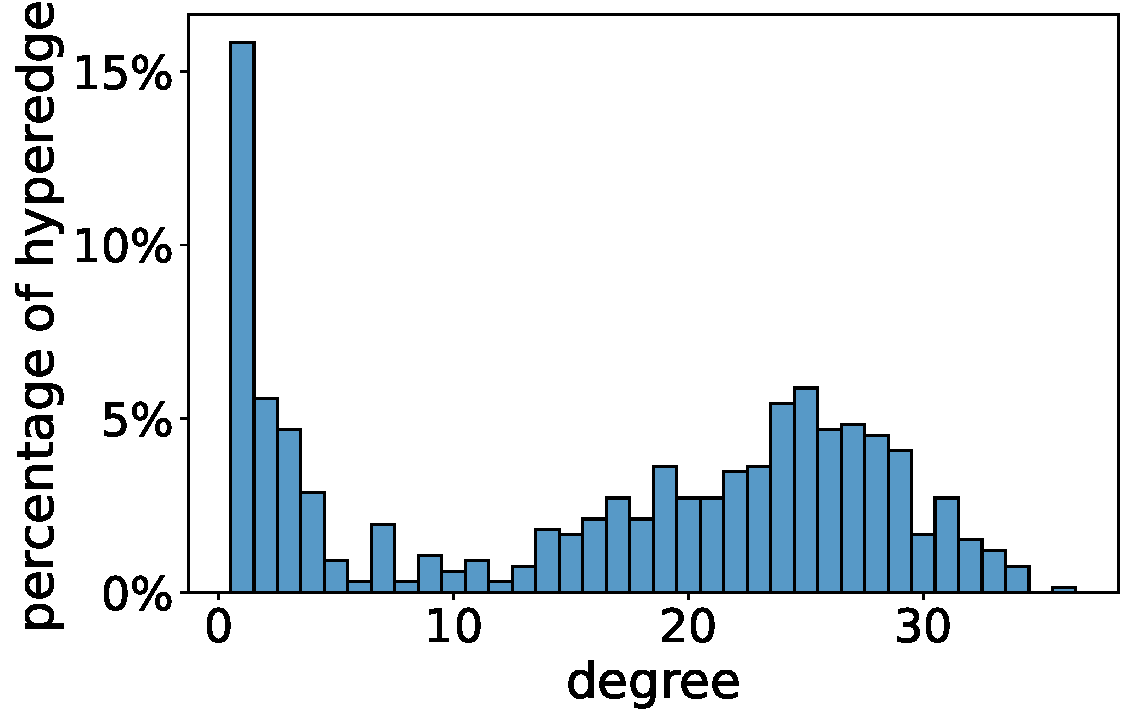
\includegraphics[width=\textwidth]{figures/degree_dist2.pdf}
        \caption{}
        \label{fig:degree_dist}
    \end{subfigure}
    \hspace{1em}
    \begin{subfigure}[t]{0.27\textwidth}
        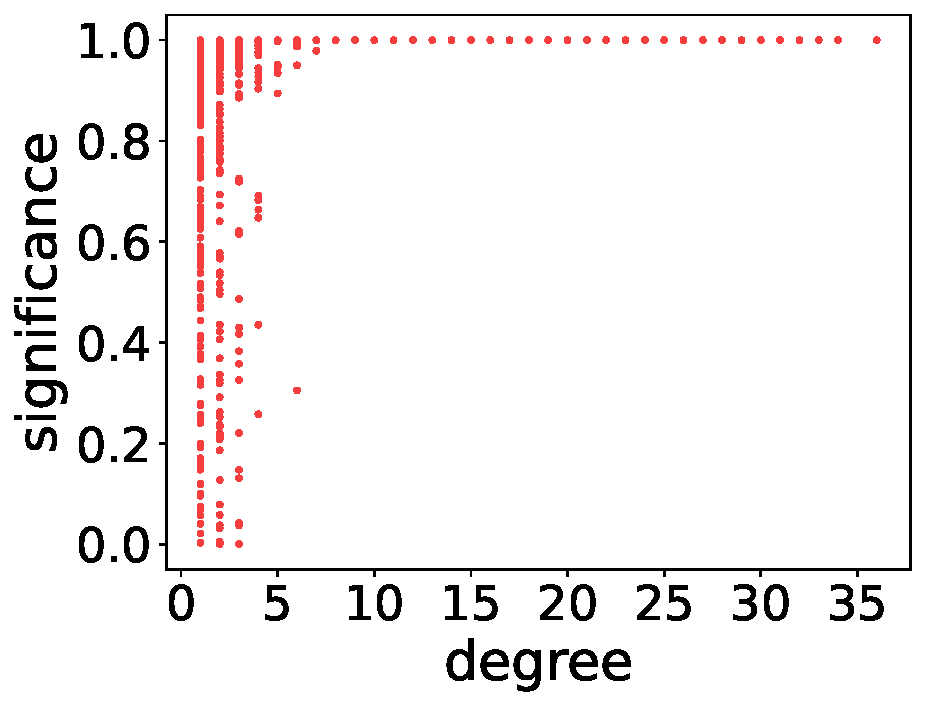
\includegraphics[width=\textwidth]{figures/degree_sig.pdf}
        \caption{}
        \label{fig:degree_sig}
    \end{subfigure}
        \hspace{1em}
    \begin{subfigure}[t]{0.28\textwidth}
        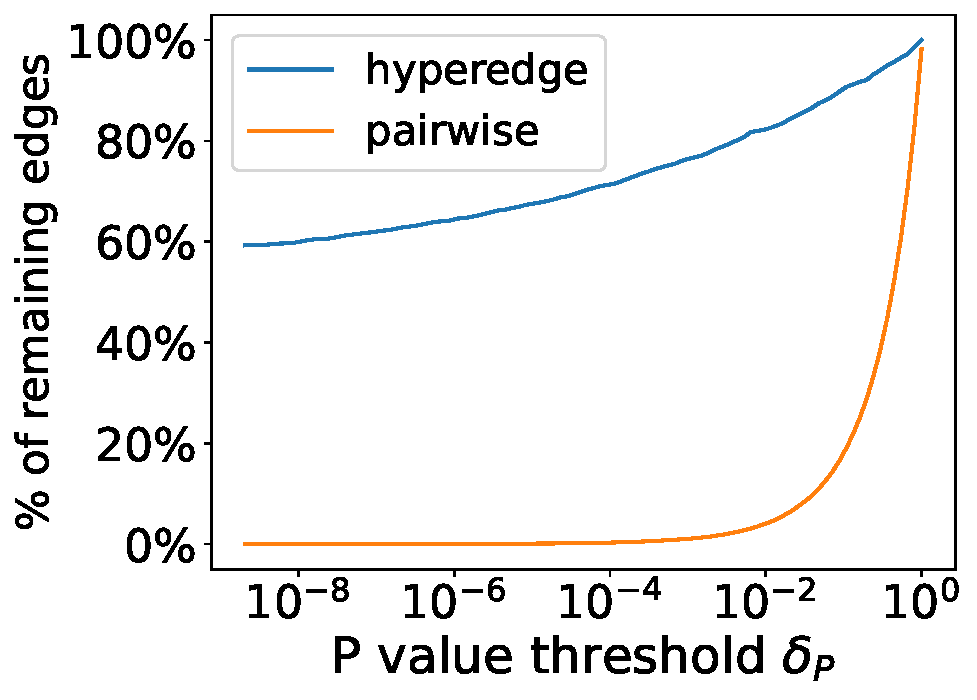
\includegraphics[width=\textwidth]{figures/num_sig.pdf}
        \caption{}
        \label{fig:cmp_sig_pair}
    \end{subfigure}
    % \vskip 0.1in
    \caption{Hyperedge profiles. \textbf{(a)} Hyperedge degree distribution of learned hyperedges. \textbf{(b)} Correlation between hyperedge degree and significance. \textbf{(c)} Comparison between the number of hyperedges and pairwise edges under different significance thresholds. The total number of hyperedges is $32$. And the total number of pairwise edges is $26,896$.}
    \label{fig:hyperedge_profile}
    % \vskip -0.1in
    \end{center}
\end{figure*}

% To further understand the relationship between hyperedge degree and its significance, we next plot their correlation in Figure \ref{fig:degree_sig}. \jialin{can be removed}
% \begin{wrapfigure}{R}{0.49\textwidth}
%           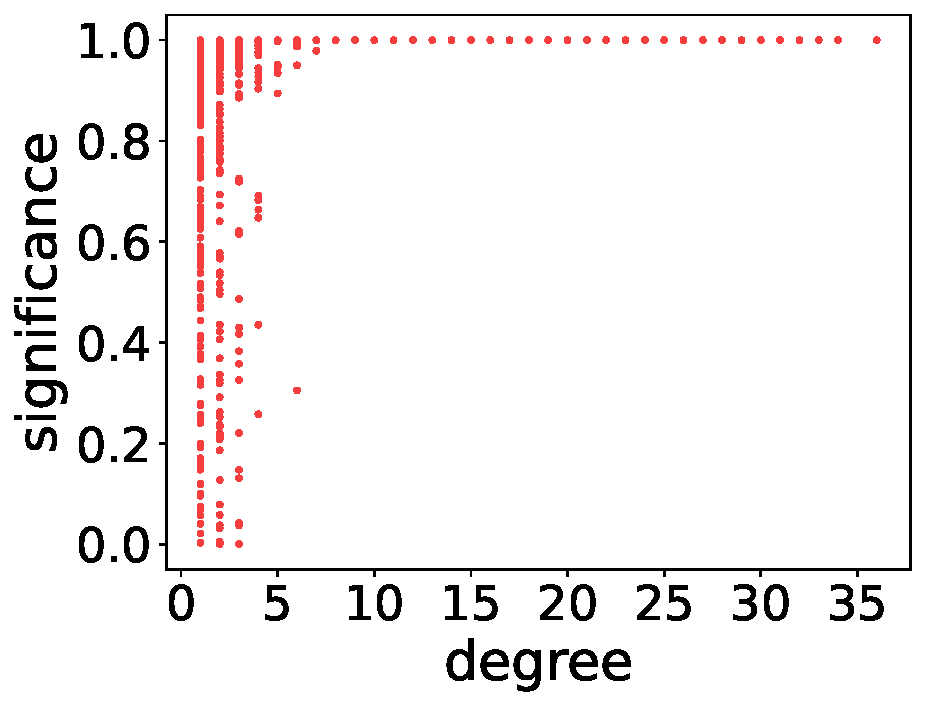
\includegraphics[width=\linewidth]{figures/degree_sig.pdf}
%     \caption{Relationship between the significances and degrees of learned hyperedges.}
%     \label{fig:degree_sig}
% \end{wrapfigure}

\paragraph{Hyperedges with Higher Degree are More Significant}
Since CPM conducts a significance test on pairwise edges and hyperedges internally based on a linear regression model, we can obtain a P-value for each hyperedge from the significance test. We define the significance of a hyperedge as $1-P_v \in [0, 1]$ where $P_v$ is the P-value of that hyperedge.

The relationship between hyperedge degree and its significance is shown in Figure ~\ref{fig:degree_sig}. In this figure, we find a strong positive correlation between a hyperedge's degree and its significance, which indicates that interactions of multiple brain regions play more important roles in cognition than pairwise or individual ones. It is also worth mentioning that there is a turning point around degree $5$, which corresponds to the valley around $5$ in Figure \ref{fig:degree_dist}.

\paragraph{High-order relationships are Better than Pairwise Ones}
To compare the significance in cognition between pairwise edges and learned hyperedges, we plot the number of remaining edges under different thresholds in Figure \ref{fig:cmp_sig_pair}. We find out that the learned hyperedges are much more significant than pairwise ones. Also note that even if we set the threshold to an extremely strict value ($1\times 10^{-8}$), there are still $60\%$ hyperedges considered significant. This evidence shows that our high-order relationships are much more significant than the traditional pairwise connectivity, which implies relationships involving multiple brain regions could be much more essential in cognition.


\paragraph{Hyperedge Case Study} We visualize the most significant hyperedge of the EN-back task in Figure \ref{fig:hyperedge1}. We observe a coordinated interaction of numerous brain regions, each fulfilling specific roles. Notably, some of these regions serve multi-functional purposes:
\begin{figure*}
    \centering
    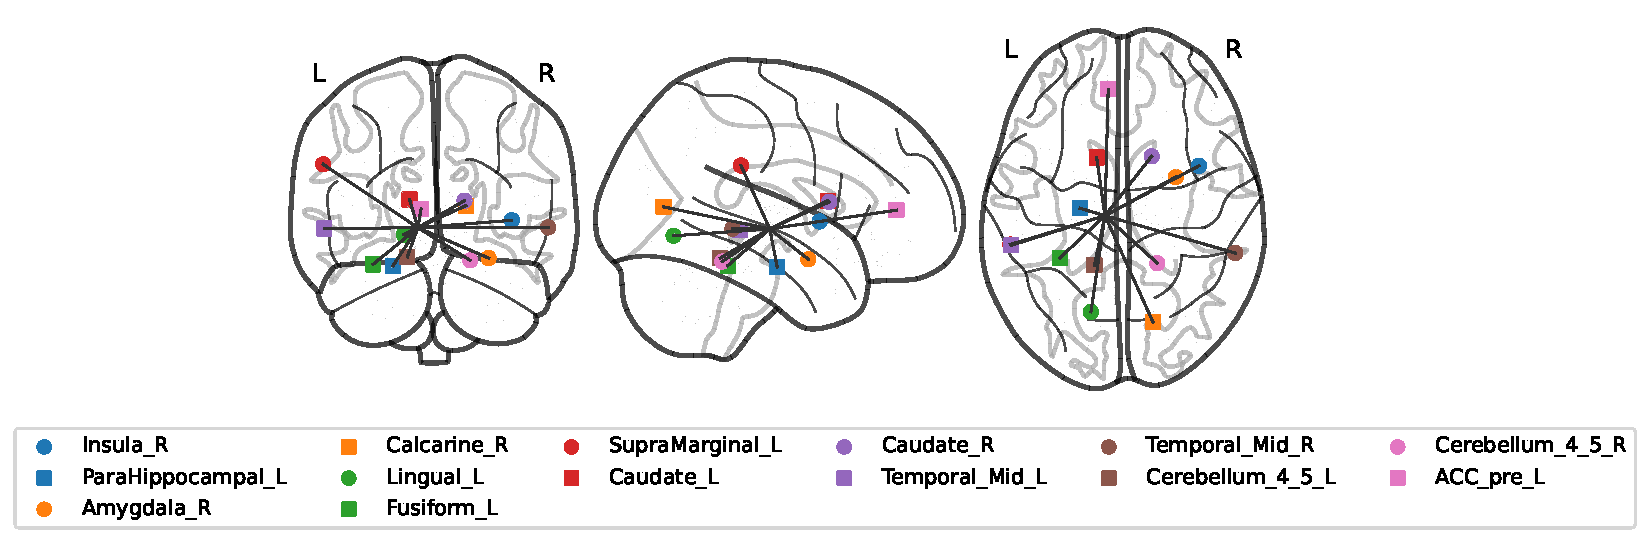
\includegraphics[width=\linewidth]{figures/hyperedge1.pdf}
    \caption{Visualization of the most significant hyperedge of the EN-back task.}
    \label{fig:hyperedge1}
\end{figure*}


\begin{itemize}
\item \textbf{Memory Processing} \textit{ParaHippocampal\_L}, \textit{Temporal Mid}: Essential for memory encoding and retrieval, these regions are integral to the EN-back task, facilitating the recall of previously viewed images.

\item \textbf{Emotional Processing} \textit{Amygdala\_R}: The amygdala is crucial for the processing of emotions, such as fear and pleasure. Since the EN-back task involves emotional stimuli, it is reasonable that the region is connected by the hyperedge.

\item \textbf{Visual Processing}: \textit{Calcarine\_R}, \textit{Lingual\_L}, \textit{Fusiform\_L}. These regions are responsible for visual perception and some of them are related to complex visual contents like symbols and human faces, which were presented during the fMRI task.

\item \textbf{Sensory} \textit{SupraMarginal\_L}: It is responsible for interpreting tactile sensors and perceiving limbs location. Its involvement is likely due to the requirement for participants to engage in specific physical actions, such as pressing buttons, during the task. \textit{Temporal Mid}: It functions in multi-modal sensory integration.

\item \textbf{Motor Control} \textit{Cerebellum}: It is primarily responsible for muscle control. \textit{Caudate}: It plays a crucial role in motor processes.  Its involvement is likely attributed to participants engaging in physical actions, like pressing buttons.

\item \textbf{Cognitive Control} \textit{ACC\_pre\_L}:  In the EN-back task, this region is likely crucial for maintaining focus, error detection and correction, conflict management in working memory, and modulating emotional responses to the task's demands.
\end{itemize}